\section{矢量数据库系统}

这一章将介绍矢量数据库系统,包括矢量数据库的架构、存储管理、安全管理和一些常见的矢量数据库系统。

\subsection{矢量数据库的架构}

\begin{figure}[H]
    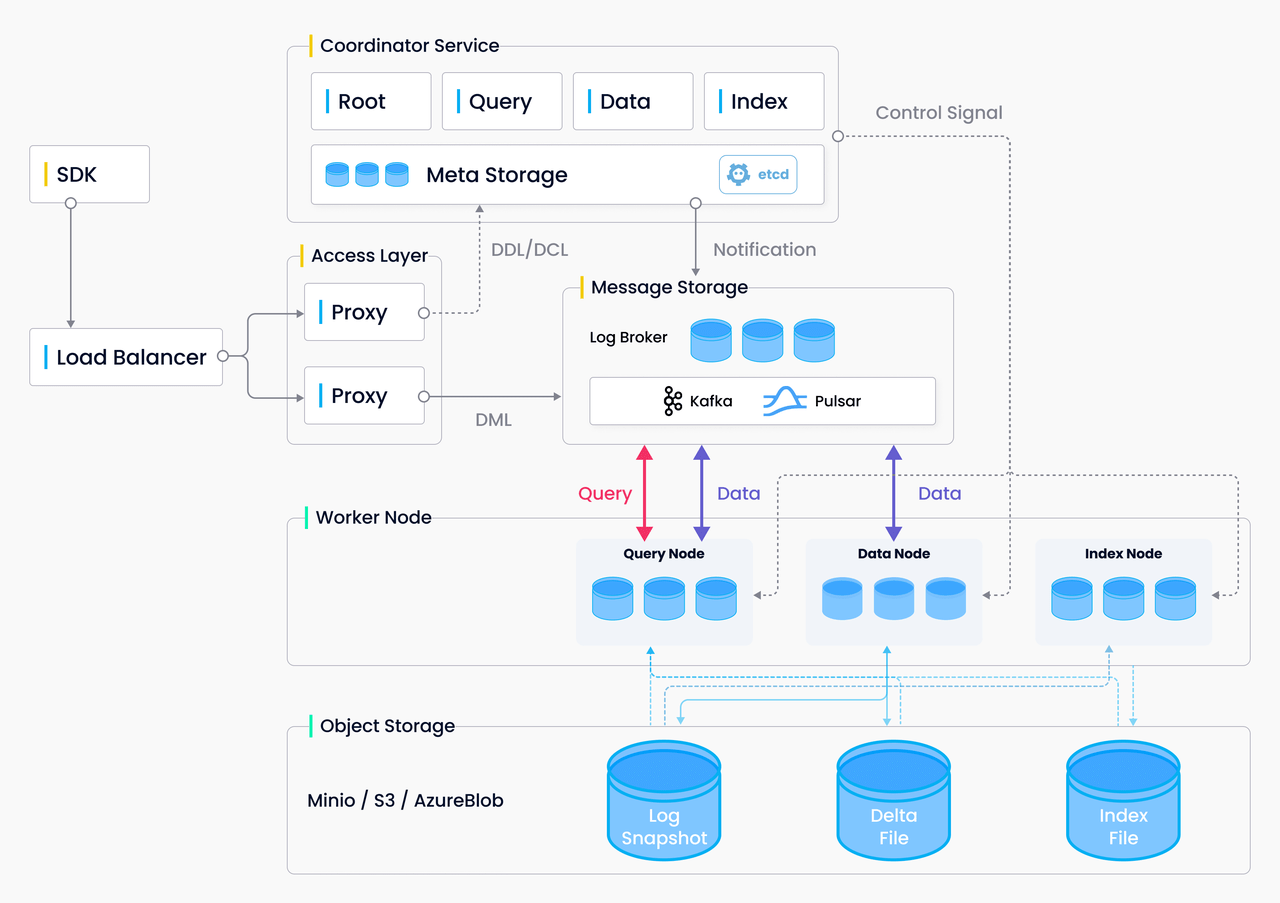
\includegraphics[width=\textwidth]{examples/arch.png}
    \centering
    \caption{Milvus矢量数据库的架构}
    \label{fig:arch}
\end{figure}

图\ref{fig:arch}展示了Milvus\cite{2021milvus}——一个现代的矢量数据库的完整架构。Milvus是一个支持数据分片、数据持久性、向量与标量混合搜索等功能的矢量数据库,采用了共享存储架构,对计算节点实现了存储和计算的分离和水平可扩展性。由于不同矢量数据库可能存在完全不同的架构,这里就以Milvus为例,介绍矢量数据库的基本架构。

Milvus采用分层架构,将整个数据库系统划分了4个层:

\begin{itemize}
    \item 访问层。访问层包含一系列无状态代理服务,是系统与用户访问之间的接口。访问层采用负载均衡组件(如Nginx、Kubernetes Ingress等)为用户提供一个统一的服务地址,并将请求分配到各个节点上。
    \item 协调服务层。协调服务层是系统的大脑,负责集群拓扑管理、负载均衡、时间戳生成、数据管理等,负责分配任务给系统节点。协调服务层中包括4个协调器:
    \begin{itemize}
        \item 根协调器,负责创建和删除节点等。
        \item 查询协调器,负责查询节点的拓扑结构和负载均衡。
        \item 数据协调器,负责维护元数据,控制后台数据的刷写、合并等操作。
        \item 索引协调器,负责构建和维护索引。
    \end{itemize}
    \item 工作节点层。工作节点层是系统中负责执行的部件,专注进行计算工作,包括3个节点:
    \begin{itemize}
        \item 查询节点,负责加载数据并执行向量/标量混合搜索。
        \item 数据节点,负责获取日志,打包快照并进行持久化。
        \item 索引节点,负责建立索引。
    \end{itemize}
    \item 持久化层。持久化层负责数据的持久化,包含元数据存储、日志代理和对象存储。
\end{itemize}

总之,现代的矢量数据库系统基本都支持分布式架构,并与分布式文件系统、对象存储等云技术结合。这是因为深度学习、大数据等领域等对大规模矢量的存储需求,单机难以承担昂贵的需求,必须要采用分布式的架构进行存储。此外,现代的矢量数据库系统通常支持多样化的功能,如矢量/标量混合查询、不同度量方式的相似度搜索等,满足用户的多样化需求。

\subsection{矢量数据库的存储管理}

基于分布式架构,数据的存储也出现各种各样的问题。可以想象的是,节点越多时,部分节点出现错误和故障的可能性就越大。因此,现代的矢量数据库必须能在各个节点随时可能宕机的情况下正常工作,满足包括查询需要尽快返回、数据不能丢失、部分节点宕机时也能正常工作等复杂需求,这对现代的矢量数据库系统提出非常高的要求。为了实现上述功能,下面将介绍现代的矢量数据库系统的存储管理策略。

Milvus1.x版本采用共享存储策略,即通过多台硬盘驱动器组成阵列来提高容量和数据安全性。一个经典的共享存储技术是RAID\cite{chen1994raid},该技术通过分片和校验等技术实现高效的读写和安全管理。

\begin{figure}[H]
    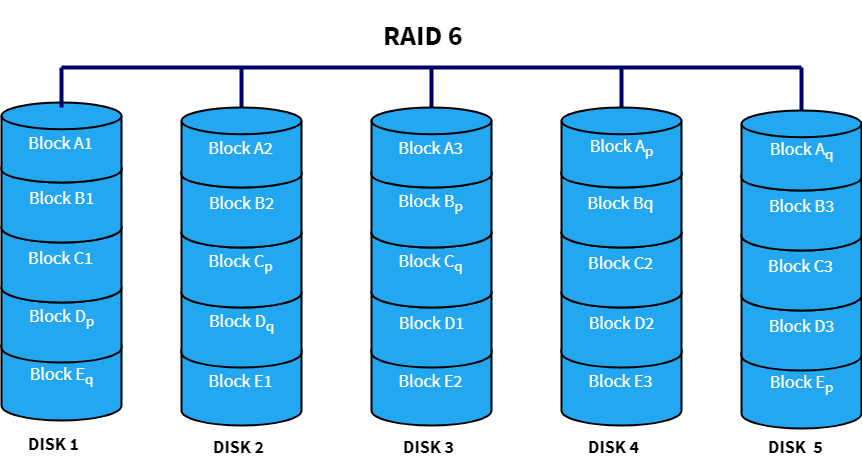
\includegraphics[width=\textwidth]{examples/raid.png}
    \centering
    \caption{RAID阵列技术}
    \label{fig:raid}
\end{figure}

如图\ref{fig:raid}所示,RAID技术将若干硬盘组成阵列,对于一条数据来说,它会被拆分为若干片,存入不同的硬盘中,这样读写数据时就可以同时读写多个硬盘,大大提高速度。另一方面,如果部分硬盘出现故障,RAID还可以通过奇偶校验\cite{gallager1962low}或异或校验等技术来恢复故障硬盘的数据。RAID 6阵列中最多支持2个硬盘发生故障,这大大提升了分布式系统的可用性。

Milvus2.0版本则直接采用云原生架构,采用云对象存储和分布式文件系统服务,由云服务厂商保障数据的安全性。

\subsection{矢量数据库的安全管理}

为了有效地管理和维护一个矢量数据库,我们需要一个强大的监控系统来跟踪数据库的性能、健康和整体状态的重要方面。监测对于检测潜在的问题、优化性能和确保顺利的生产运营至关重要。通常一个矢量数据库需要支持如下数据的监控:

\begin{itemize}
    \item 资源使用情况。监测资源使用情况,如 CPU、内存、磁盘空间和网络活动,可以识别可能影响数据库性能的潜在问题或资源限制。
    \item 查询性能。查询延迟、吞吐量和错误率可能表明需要解决的潜在系统性问题。
    \item 系统健康。整体系统健康监测包括单个节点、复制过程和其他关键组件的状态。
\end{itemize}

此外,为了保证用户安全,矢量数据库需要支持用户权限的访问控制,确保只有授权用户才有能力查看、修改、存储库中的部分敏感数据,避免数据丢失和财产损失。

最后,为了保证数据安全,矢量数据库需要提供定期备份的功能,备份数据存储在外部系统中,与数据库存储分离,确保数据的安全性和可恢复性。当数据发生丢失和损坏时,这些备份可以用来将数据库恢复到以前的状态,最大限度地减少停机时间和对整个系统的影响。

Milvus支持了上述提到了监控、权限管理、数据备份等功能,拥有丰富的安全管理机制,能够保证安全性。

\subsection{一些常见的矢量数据库系统}

以下是一些流行的矢量数据库系统:

\begin{itemize}
    \item Milvus。Milvus是一个开源矢量数据库,可以管理万亿矢量数据集,支持多种矢量搜索索引和内置过滤。
    \item Pinecone。Pinecone是一个专为机器学习应用程序设计的矢量数据库。它速度快、可扩展,并支持多种机器学习算法。Pinecone建立在Faiss之上,Faiss是一个用于密集向量高效相似性搜索的库。
    \item Faiss。Faiss库是由Facebook开发的适用于稠密向量匹配的开源库,支持多种向量检索方式,包括内积、欧氏距离等,同时支持精确检索与模糊搜索.
    \item Annoy。Annoy是一个C++库,用于在高维空间中搜索最近邻居。它支持欧几里得距离和曼哈顿距离,并且可以使用多个CPU核心进行计算。
    \item Hnswlib。Hnswlib是一种快速、可扩展和高效的近似最近邻居搜索库。它支持多线程计算,并且可以在大型数据集上进行分布式计算。
\end{itemize}
